
\section{Grain charging and gas--grain coupling around OB stars}
\label{sec:cloudy-models-dust}

We calculate models of the physical properties of dust grains using
the plasma physics code Cloudy \citep{Ferland:2013a, Ferland:2017a},
which self-consistently solves the multi-frequency radiative transfer
together with thermal, ionization, and excitation balance of all
plasma constituents.  Cloudy incorporates grain charging as described
in \citet{Baldwin:1991a} and \citet{van-Hoof:2004a} with photoelectric
emission theory from \citet{Weingartner:2001b, Weingartner:2006a}.  We
use the default ``ISM'' dust mixture included in Cloudy, which
comprises ten size bins each for spherical silicate and graphite
grains in the range \num{0.005} to \SI{0.25}{\um}, and which is
designed to reproduce the average Galactic extinction curve
\citep{Weingartner:2001a, Abel:2008a}.  The optical properties of each
grain species are calculated using Mie theory \citep{Bohren:1983a},
assuming solid spheres.  The resultant wavelength-dependent extinction
properties of the mixture are summarised in
Figure~\ref{fig:cloudy-ism-dust-opacity}.

\begin{figure}
  \centering
  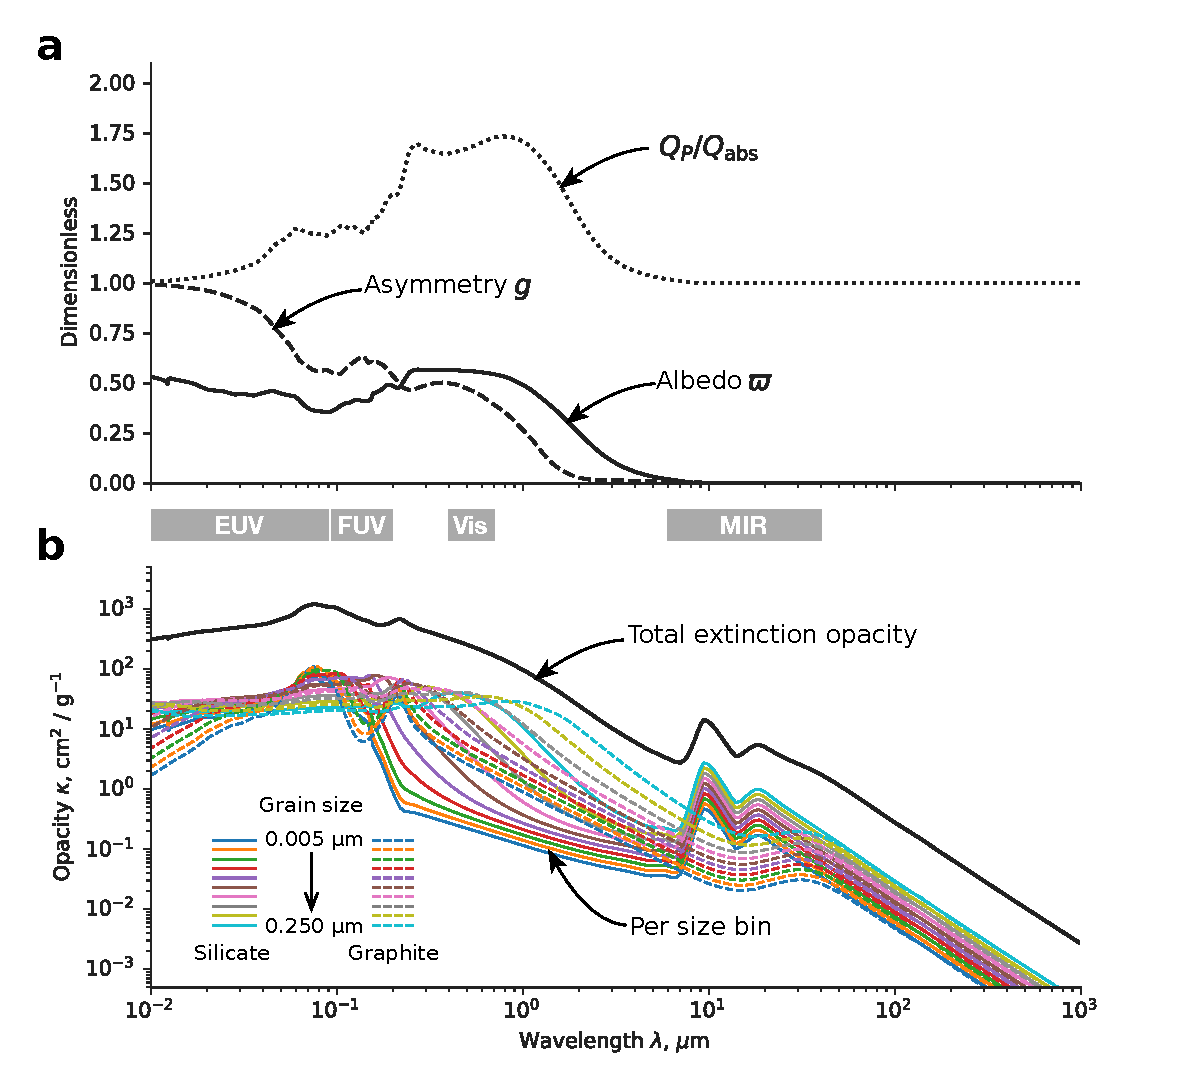
\includegraphics[width=\linewidth]{figs/cloudy-ism-dust-opacity}
  \caption{Extinction properties of Cloudy's standard ``ISM'' dust
    mixture. %
    (a)~Wavelength dependence of mean values over the entire mixture
    of three dimensionless quantities related to scattering: albedo,
    \(\varpi\) (solid line); scattering asymmetry,
    \(g = \langle \cos\theta \rangle\) (dashed line); ratio of radiation pressure
    efficiency to absorption efficiency, \(Q_P / Q_{\text{abs}}\)
    (dotted line).
    %
    (b)~Wavelength dependence of mass opacity (cross section per unit
    mass of gas) for the whole mixture (heavy black line) and broken
    down by size bin and grain composition (colored lines, see key). }
  \label{fig:cloudy-ism-dust-opacity}
\end{figure}

To ascertain the expected variation in grain properties in the
circumstellar environs of luminous stars, we calculate a series of
spherically symmetric, steady-state, constant density Cloudy simulations,
illuminated by the stars listed in Table~\ref{tab:stars}, with stellar
spectra taken from the OSTAR2002 and BSTAR2006 grids, calculated with
the TLUSTY model atmosphere code \citep{Lanz:2003a, Lanz:2007a}.
Simulations are run for hydrogen densities of
\numlist{1;10;100;e3;e4} \si{cm^{-3}} and assuming standard \hii{} region
gas phase abundances.  The calculation is stopped when the ionization
front is reached and the inner radius is chosen to be roughly 1\% of this. 



\begin{figure*}
  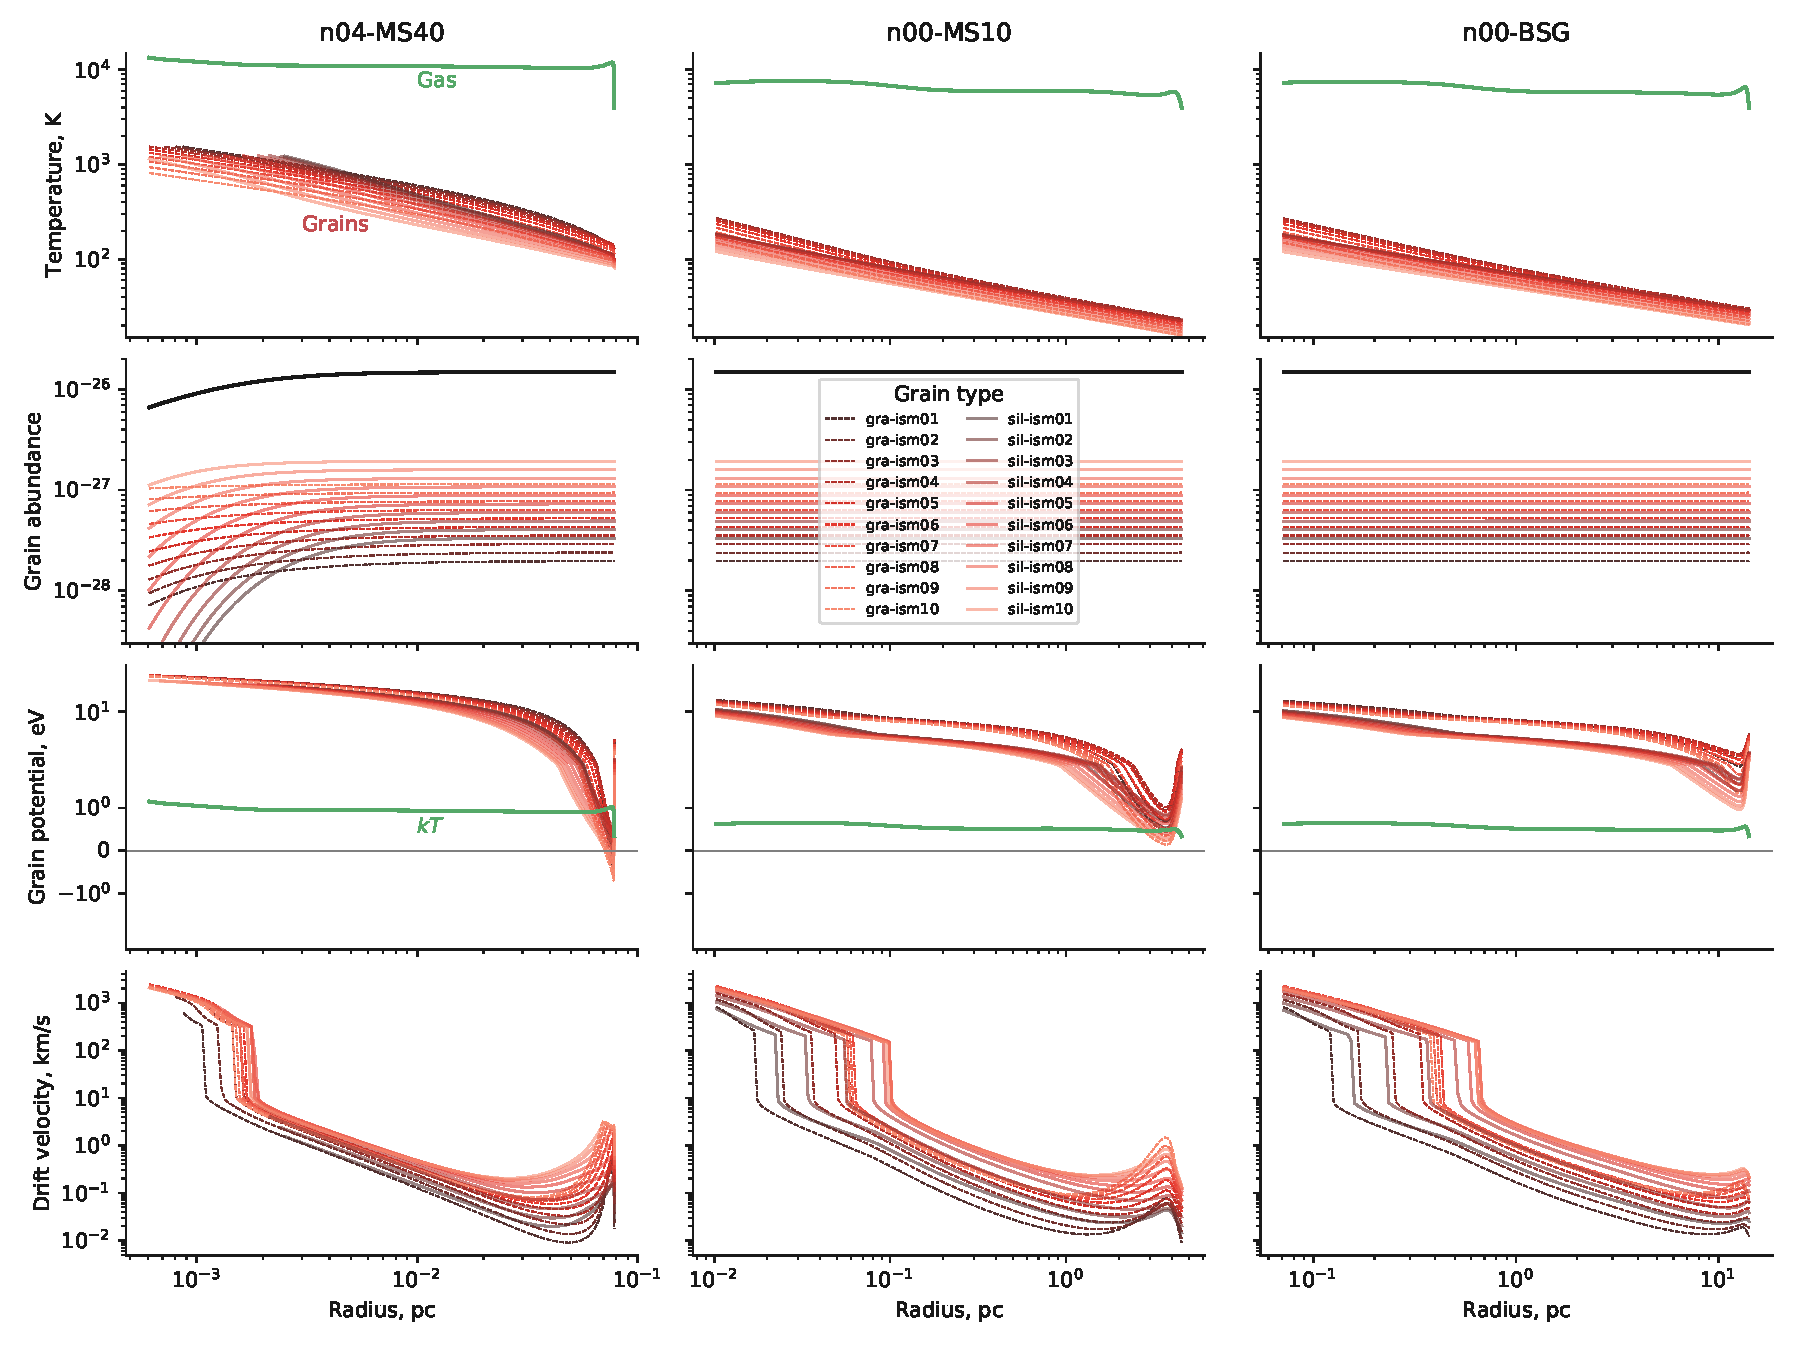
\includegraphics[width=\linewidth]{figs/multi-dustprops}
  \caption{Dust properties as a function of radius from star for three
    selected Cloudy simulations. (a)~\SI{40}{M_\odot} main-sequence star in
    medium of density \SI{e4}{cm^{-3}}. (b)~\SI{10}{M_\odot} main-sequence
    star in medium of density \SI{1}{cm^{-3}}. (c)~Blue supergiant
    star in medium of density \SI{1}{cm^{-3}}}.
  \label{fig:multi-dustprops}
\end{figure*}
Figure~\ref{fig:multi-dustprops} shows resultant radial profiles of
dust properties for representative simulations: grain temperature, grain
abundance, grain potential, and grain drift velocity.  Line types
correspond to the different size bins of graphite and silicate grains,
as indicated in the key from smallest to largest. The left hand panels
show results for a high-density (\(n = \SI{e4}{cm^{-3}}\)), compact
(\(R \approx \SI{0.1}{pc}\)) region around an early O~star, where the grain
temperature is very high, especially for the smaller silicate grains,
and sublimation significantly reduces the grain abundance in the inner
regions.  The remaining columns show low-density
(\(n = \SI{1}{cm^{-3}}\)), extended (\(R \sim \SI{10}{pc}\)) regions
around main-sequence and supergiant B-type stars, in which the grain
temperatures are much lower, ranging from \SIrange{20}{50}{K} in the
outer parts up to \SIrange{100}{200}{K} in the inner parts.

 
\begin{figure*}
  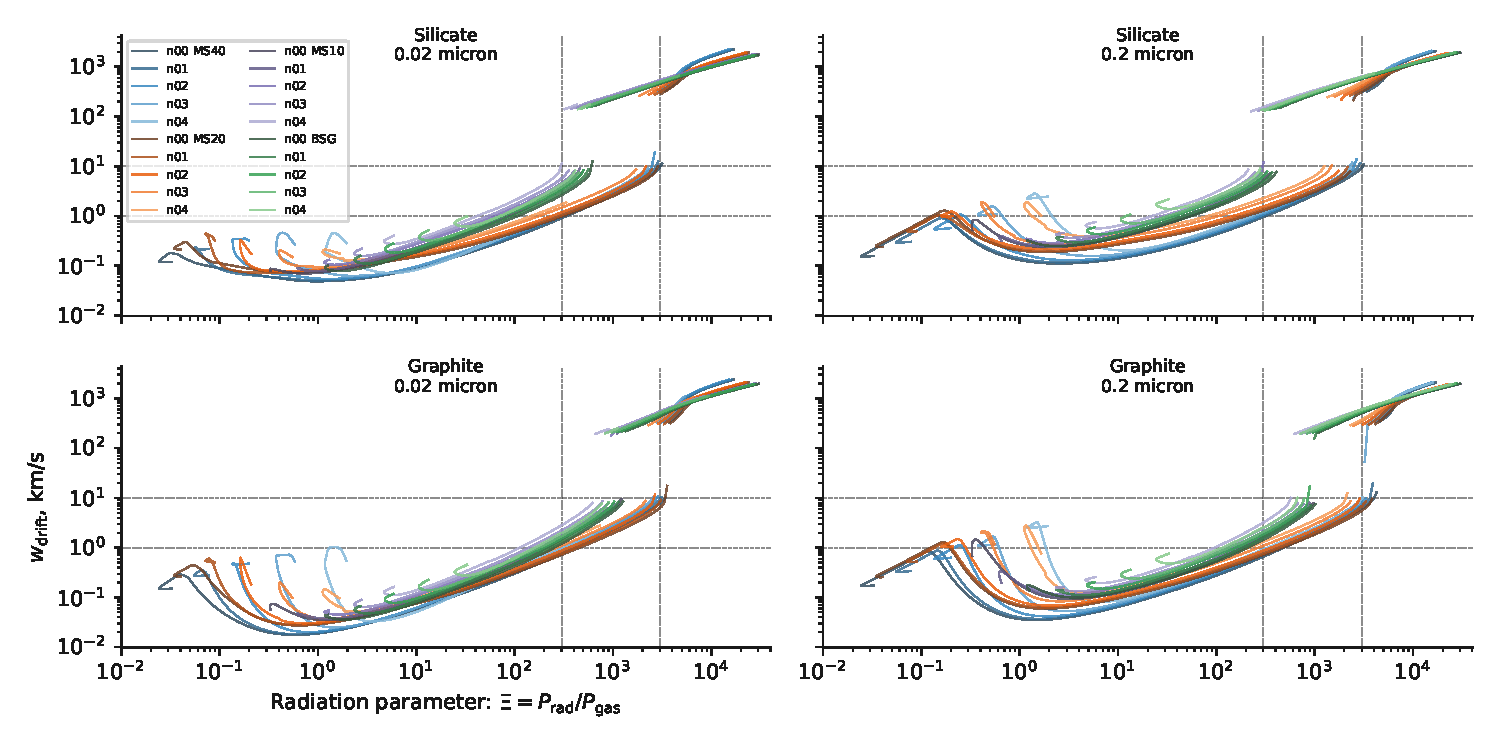
\includegraphics[width=\linewidth]{figs/drift-pratio-4panel}
  \caption{Drift velocity \(w\drift\) versus radiation parameter
    \(\Xi\). Each line represents a simulation with ambient density and
    stellar type as indicated in the key.  Results are shown for
    graphite and silicate grains of two different sizes.  The rip
    point, which corresponds to gas--grain decoupling, is the
    discontinuity in the curves at
    \(w\drift \approx \SI{10}{km.s^{-1}}\), indicated by the upper
    horizontal dashed line.  The vertical dashed lines show the narrow
    range of radiation parameter, \(\Xi = 1000 \pm \SI{0.5}{dex}\), that
    encompasses the rip point for all simulations. }
  \label{fig:drift-gn}
\end{figure*}

Unlike the strong differences in thermal properties, the radial
dependence of grain electrostatic potential (third row in
Fig.~\ref{fig:multi-dustprops}) is qualitatively similar for all the
simulations.  The grains are predominantly positively charged, with high
potentials (\(> 10\) times the thermal energy of gas particles) close
to the star due to the strong EUV and FUV photo-ejection.  The
potential falls to much lower values in the outer ionized region, as
the EUV flux falls off, and then climbs again at the ionization front
due to the fall in electron density, while the FUV photo-ejection
persists well into the neutral region.  There are small differences
between the simulations due to the increasing relative importance of the
EUV radiation for hotter stars, which leads to a deeper dip in the
potential just inside the ionization front for the \SI{40}{M_\odot} case,
even reaching negative values for some grain species.

Equilibrium drift velocity for each grain species is calculated in the
Cloudy simulations using the same theory \citep{Draine:1979a} as
outlined in \S~\ref{sec:drag-force-grains}.  The way that this is
implemented by default in Cloudy means that if the only solution at
the inner radius is a superthermal one, then the superthermal solution
branch (upper right corner of
Fig.~\ref{fig:gas-grain-drag-photoionized}) is followed as far as
possible through the outer spatial zones.  We have modified the code
so as to instead always prefer the slower subthermal branch whenever
multiple solutions are available.  This makes the most sense in our
context, where the grains are moving towards the star and so the
radiative force is gradually increasing from an initial low value.
Example results are shown in the bottom row of
Figure~\ref{fig:multi-dustprops} and again they are qualitatively
similar for all the simulations.  Close to the star, the radiation
force is higher than the upper limit on the Coulomb drag force
(eq.~[\ref{eq:fdrag-maximum}]), so that the equilibrium drift velocity
is exceedingly high.\footnote{Note that such high drift velocities are
  much higher than any realistic true relative velocity between grains
  and gas, since they are based on the assumption that the radiation
  force remains constant while the grain is accelerated, which is not
  the case near the rip point.  Instead, they are simply an indication
  that the gas and grains have completely decoupled.}.  As the radial
distance from the star increases, the radiation field is increasingly
diluted but the grain potential falls only slowly, so eventually one
reaches a point where an equilibrium between Coulomb drag and
radiation force can be established, which corresponds to a
discontinuity in the drift velocity.  This is the \textit{rip point}
discussed in \S~\ref{sec:gas-grain-separ}.  The drift velocity carries
on falling towards the outside of the \hii{} region, but then
increases again just inside the ionization front due to the drop in
grain potential there.

Both the charge balance and the force balance are essentially due to
competition between the photons and the charged particles that
interact with the grain.  It is therefore reasonable to surmise that
the gas--grain decoupling that occurs at the rip point might be
determined principally by the ratio of photons to gas particles.  We
test this hypothesis in Figure~\ref{fig:drift-gn}, where we
characterize the photon-gas ratio by a dimensionless radiation
parameter, \(\Xi\), equal to the radiation pressure divided by the gas
pressure.  Results are shown for four different grain types and for
all combinations of stellar parameters and ambient densities for which
we have run simulations.  It can be seen that the rip point does indeed
always occur at a similar value of \(\Xi \sim 1000\) for all simulations, albeit
with some variation according to the spectral type of the star and the
grain composition, as given in Table~\ref{tab:Xi-rip}.  The gas
density and grain size have very little influence on this critical
value \(\Xi_\dag\), with the only exception being the very smallest grains
(\(a < \SI{0.006}{\um}\), not illustrated), which show
\(\Xi_\dag \approx \num{e4}\), but such grains are only minor contributors to the
UV opacity (\(< 10\%\) in EUV and \(< 1\%\) in FUV, see
Fig.~\ref{fig:cloudy-ism-dust-opacity}).

\begin{figure}
  \centering
  \includegraphics[width=\linewidth]{figs/phi-versus-xi-annotate}
  \caption{Grain potential in thermal units (linear scale) versus
    radiation parameter (logarithmic scale). All densities and stellar
    types are shown, with line colors as in Fig.~\ref{fig:drift-gn}.
    Solid lines show silicate grains and dashed lines show graphite
    grains.  Line width increases with grain size (to reduce clutter,
    only every second size bin is shown).  The solid and dashed lines
    show the logarithmic fits discussed in the text.}
  \label{fig:phi-vs-Xi}
\end{figure}
Finally, Figure~\ref{fig:phi-vs-Xi} shows the slow dependence of grain
potential on radiation parameter for all the simulations on a linear
versus logarithmic scale.  The logarithmic fit of
equation~\eqref{eq:phi-vs-Xi}, most appropriate for carbon grains
around cooler stars, is shown by the solid line.  The dashed lines
show the modifications for silicate grains and for hotter stars (see
\S~\ref{sec:gas-grain-separ}).  Further details of the Cloudy dust
models are discussed in Appendix~\ref{sec:grain-temp-emiss}.

\section{Grain temperature and mid-infrared emissivity}
\label{sec:grain-temp-emiss}


\begin{figure}
  \centering
  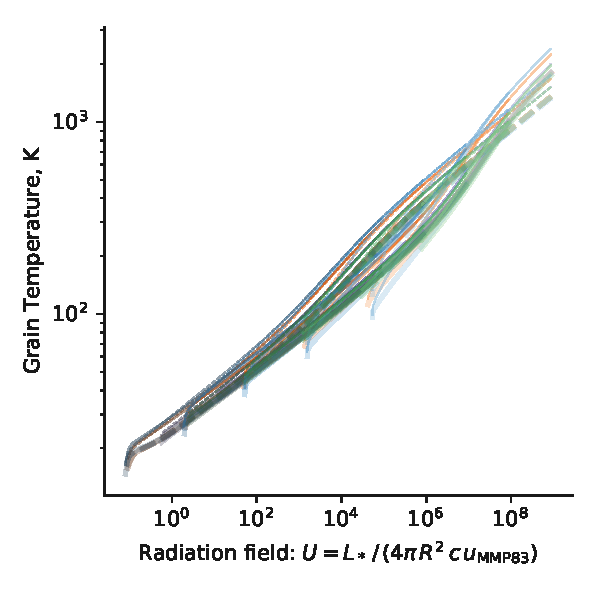
\includegraphics[width=\linewidth]{figs/grain-T-vs-U}
  \caption{Grain temperature versus radiation field mean intensity,
    \(U\), in units of the interstellar radiation field in the solar
    neighborhood.  Line types and colors are as in
    Fig.~\ref{fig:phi-vs-Xi} and correspond to a variety of stellar
    spectral shapes, gas densities, and grain species.}
  \label{fig:grain-T-vs-U}
\end{figure}

Figure~\ref{fig:grain-T-vs-U} shows equilibrium grain temperatures for
the Cloudy models discussed in Appendix~\ref{sec:cloudy-models-dust}
as a function of the nominal energy density of the radiation field,
\(U = u / u\mmp \), where \(u = L / 4 \pi R^2 c\) and \(u\mmp\) is the
energy density of the interstellar radiation field for
\(\lambda < \SI{8}{\um}\) in the solar neighborhood
\citep{Mathis:1983a}:
\begin{equation}
  \label{eq:u-mmp83}
  u\mmp\,c = \SI{0.0217}{erg.s^{-1}.cm^{-2}} \ .
\end{equation}
The tight relationship seen in figure~\ref{fig:grain-T-vs-U} between
\(T\) and \(U\) is evidence for the dominance of stellar radiative
heating (see \S~\ref{sec:unimp-other-heat} below), while the variation
about the mean relation is mainly due to differences in grain size and
composition, with smaller grains and graphite grains being relatively
hotter.  The downward hooks seen on the left end of each simulation's
individual curve are due to the fact that our calculation of \(U\)
does not account for internal absorption, which starts to become
important near the ionization front.

\begin{figure}
  \centering
  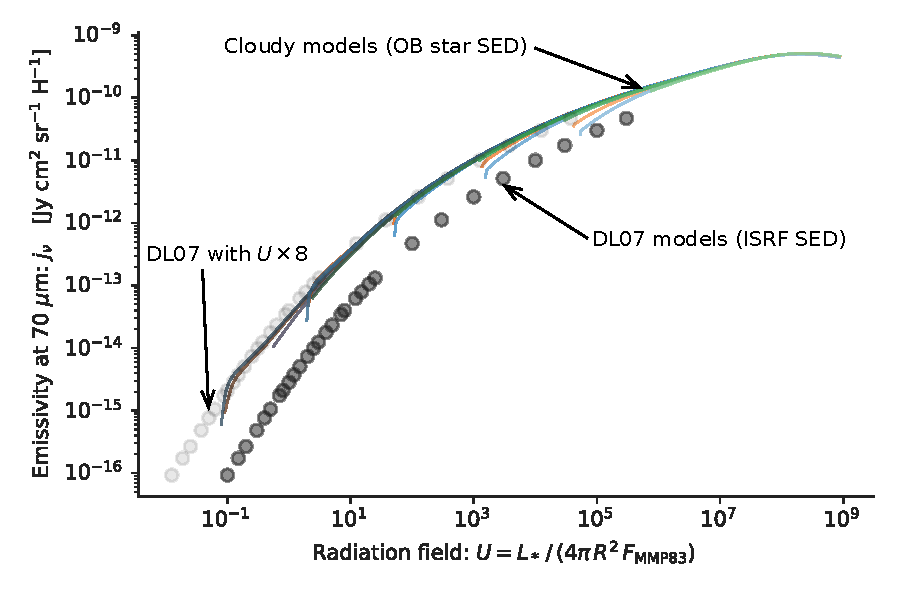
\includegraphics[width=\linewidth]{figs/grain-j70-vs-U-edited}
  \caption{Grain emissivity at \SI{70}{\um} for all Cloudy models
    (lines colored as in Fig.~\ref{fig:drift-gn}), compared with grain
    models from \citet{Draine:2007a} (dark gray symbols), which assume
    illumination by a scaled interstellar radiation field, which has a
    SED with a very different shape from that of an OB star, see
    Fig.~\ref{fig:sed-comparison}.  }
  \label{fig:grain-j70}
\end{figure}

The grain emissivity at \SI{70}{\um} (Herschel PACS blue band) for the
Cloudy simulations (colored lines) is shown in
Figure~\ref{fig:grain-j70}, where it is compared with the same
quantity from the grain models (dark gray symbols) of
\citet{Draine:2007a}.  A clear difference is seen between the two sets
of models, but this is due almost entirely to a difference in the
assumed spectrum of the illuminating radiation, as illustrated in
Figure~\ref{fig:sed-comparison}.  \citet{Draine:2007a} use a SED that
is typical of the interstellar radiation field in the Galaxy, which is
dominated by an old stellar population, which peaks in the near
infrared, with only a small FUV contribution from younger stars (about
8\% of the total energy density).  This is very different from the OB
star SEDs, which are dominated by the FUV and EUV bands.  Since the
grain absorption opacity is much higher at UV wavelengths than in the
visible/IR (see Fig.~\ref{fig:cloudy-ism-dust-opacity}), the effective
grain heating efficiency of the OB star SED is correspondingly higher.
The light gray symbols show the effect on the \citet{Draine:2007a}
models of multiplying the radiation field by a factor of \num{8} in
order to offset this difference in efficiency, which can be seen to
bring them into close agreement with the Cloudy models.  A further
difference is that the \citet{Draine:2007a} model includes small PAH
particles, which we do not include in our Cloudy models, since they
are believed to be largely absent in photoionized regions
\citep{Giard:1994a, Lebouteiller:2011a}.  However, this only effects
the emissivity at shorter mid-infrared wavelengths \(< \SI{20}{\um}\).

\begin{figure}
  \centering
  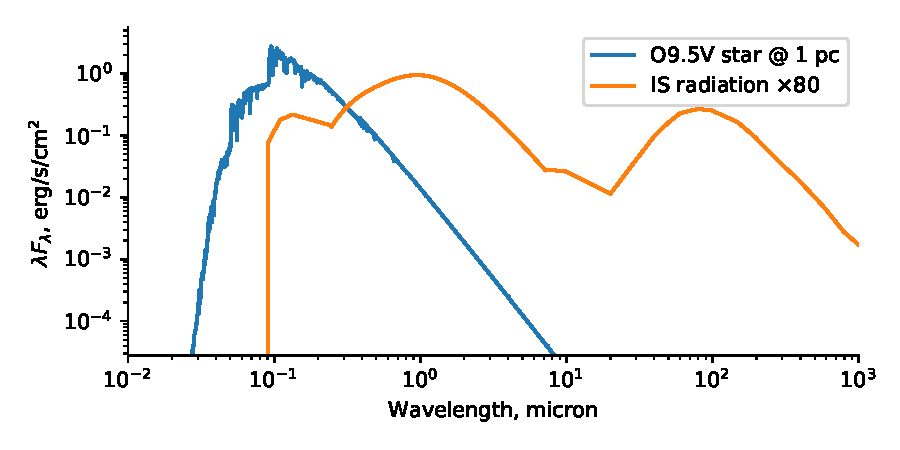
\includegraphics[width=\linewidth]{figs/sed-comparison}
  \caption{Comparison between the spectral energy distribution (SED)
    of a typical OB star (blue line) and the interstellar radiation
    field in the solar neighborhood (orange line).  The OB star is the
    \SI{20}{M_\odot} model from Table~\ref{tab:stars} and is plotted for a
    distance from the star of \SI{1}{pc}.  The interstellar SED is
    from \citet{Mathis:1983a} and is multiplied by \num{80} so that
    the total FUV-to-NIR flux is equal for the two SEDs.}
  \label{fig:sed-comparison}
\end{figure}

In terms of the characteristic parameters introduced in
\S~\ref{sec:depend-stell-type} the dimensionless radiation field becomes
\begin{equation}
  \label{eq:U-from-L4-and-Rpc}
  U = 14.7\, L_4\, R_{\text{pc}}^{-2} \ ,
\end{equation}
or, alternatively, it can be expressed in terms of the ambient stream as
\begin{equation}
  \label{eq:U-from-ambient}
  U = 3.01 \, n \, v_{10}^2 / x^2 \ , 
\end{equation}
where \(x = R_0/R_*\) is given by equation~\eqref{eq:x-cases}.  It can
also be related to the radiation parameter \(\Xi\), defined in
equation~\eqref{eq:Xi-Prad-over-Pgas}, as
\begin{equation}
  \label{eq:U-vs-Xi}
  U = 3.82 \, n T_4 \, \Xi \ .
\end{equation}
A common alternative approach to scaling the radiation field (see
\citealp{Tielens:1985a} and citations thereof) is to normalize in the
FUV band (\SIrange{0.0912}{0.24}{\um}), where the local interstellar
value is known as the Habing flux \citep{Habing:1968a}:
\begin{equation}
  \label{eq:Habing-flux}
  F\Hab = \SI{0.0016}{erg.s^{-1}.cm^{-2}} \ .
\end{equation}
The resultant dimensionless flux is often denoted by \(G_0\), and the
relationship between \(G_0\) and \(U\) depends on the fraction
\(f_{\text{fuv}}\) of the stellar luminosity that is emitted in the
FUV band:
\begin{equation}
  \label{eq:G-vs-U}
  G_0 = f_{\text{fuv}} \frac{u\mmp\, c}{F\Hab} \,U = (\text{\numrange{6}{10}}) \,U \ ,
\end{equation}
where we give the range corresponding to early O (\(f_{\text{fuv}} \approx 0.4\)) to early B (\(f_{\text{fuv}} \approx 0.7\)) stars.

%% Single-photon heating of small grains

\subsection{Unimportance of other heating mechanisms}
\label{sec:unimp-other-heat}
The grain temperature in bows around OB stars is determined
principally by the steady-state equilibrium between the absorption of
stellar UV radiation (heating) and the thermal emission of infrared
radiation (cooling).  Other processes such as single-photon stochastic
heating, Lyman~\(\alpha\) line radiation, and post-shock collisional
heating can dominate in other contexts, but these are generally
unimportant for circumstellar bows, as we now demonstrate.

\subsubsection{Stochastic single-photon heating}

When the radiation field is sufficiently dilute, then a grain that
absorbs a photon has sufficient time to radiate all that energy away
before it absorbs another photon \citep{Duley:1973a}.  In this case,
the emitted infrared spectrum for \(\lambda < \SI{50}{\um}\) becomes
relatively insensitive of the energy density of the incident radiation
\citep{Draine:2001a}.  However, this is most important for the very
smallest grains.  From equation~(47) of \citet{Draine:2001a}, one
finds that grains with sizes larger than
\(a = \SI{0.005}{\um} = \SI{5}{nm}\) (the smallest size included in
our Cloudy models) should be close to thermal equilibrium for
\(U > 30\), which is small compared with typical bow shock values
(\(U = \text{\numrange{e3}{e6}}\)).  As mentioned above, PAHs are not
expected to be present in the interior of \hii{} regions.
\citealp{Desert:1990a} found them to be strongly depleted for
\(U > 100\) around O stars.  However, other types of ultra-small
grains, down to sub-nm sizes \citep{Xie:2018a} may be present in bows,
and stochastic heating \emph{would} be important for grains with
\(a = \SI{1}{nm}\) if \(U < \num{e5}\).  Note, however that grains
smaller than \SI{0.6}{nm} would be destroyed by sublimation after
absorbing a single He-ionizing photon.


\subsubsection{Lyman \(\alpha\) heating}

On the scale of an entire \hii{} region, the dust heating is typically
dominated by Lyman \(\alpha\) hydrogen recombination line photons, which
are trapped by resonant scattering (e.g., \citealp{Spitzer:1978a}
\S~9.1b).  However, this is no longer true on the much smaller scale
of typical bow shocks.  An upper limit on the Lyman \(\alpha\) energy
density can be found by assuming all line photons are ultimately
destroyed by dust absorption rather than escaping in the line wings
(e.g., \citealp{Henney:1998b}), which yields
\begin{equation}
  \label{eq:U-Lya}
  U\Lya \approx 0.1 n / \kappa_{600} \ .
\end{equation}
This can be combined with equation~\eqref{eq:U-from-ambient} to give
the ratio of Lyman \(\alpha\) to direct stellar radiation as
\begin{equation}
  \label{eq:Lya-over-stellar}
  \frac{U\Lya}{U} \approx 0.03 \frac{x^2}{v_{10}^2 \kappa_{600}} \ .
\end{equation}
Taking the most favorable parameters imaginable of a slow stream
(\(v_{10} = 2\)), very strong wind (\(x \approx 1\)), and reduced dust
opacity (\(\kappa_{600} = 0.1\)) gives a Lyman \(\alpha\) contribution of only
10\% of the stellar radiative energy density.  In any other
circumstances, the fraction would be even lower.

\subsubsection{Shock heating}
\newcommand\kin{\ensuremath{_{\text{kin}}}}
The outer shock thermalizes the kinetic energy of the ambient stream,
which may in principle contribute to the infrared emission of the bow.
In order for this process to be competitive, the following three
conditions must all hold:
\begin{enumerate}[1.]
\item The post-shock gas must radiate efficiently with a cooling
  length less than the bow size, see \S~\ref{sec:radi-cool-lengths}.
  This is satisfied for all but the lowest densities (see
  Fig.~\ref{fig:zones-v-n-plane}).
\item A significant fraction of the shock energy must be radiated by
  dust.  This requires that the post-shock temperature be greater than
  \SI{e6}{K}, which requires a stream velocity
  \(v > \SI{200}{km.s^{-1}}\) \citep{Draine:1981a}.  This also
  coincides with the range of shock velocities where the smaller
  grains will start to be destroyed by sputtering in the post-shock
  gas.
\item The kinetic energy flux through the shock must be significant,
  compared with the fraction of the stellar radiation flux that is
  absorbed and reprocessed by the bow shell.
\end{enumerate}
It turns out that the third condition is the most stringent, so we
will consider it in detail.  The kinetic energy flux through the outer shock for an ambient stream of density \(\rho\) and velocity \(v\) is
\begin{equation}
  \label{eq:Fkin}
  F\ke = \tfrac12 \rho v^3 = \tfrac12 P\shell v \ , 
\end{equation}
while the stellar radiative energy flux absorbed by the shell is
\begin{equation}
  \label{eq:Ftrap}
  F\trap \approx \tau L / 4 \pi R_0^2 \ ,
\end{equation}
assuming an absorption optical depth \(\tau \ll 1\). The shell
pressure in the WBS case can be equated to the ram pressure of the
internal stellar wind (see \S~\ref{sec:three-bow-regimes}), so that
the ratio of the two energy fluxes is
\begin{equation}
  \label{eq:F-ratio-shock}
  \frac{F\ke}{F\trap} = \frac12 \frac{\eta\wind}{\tau} \frac{v}{c} \ .
\end{equation}
An upper limit to the stellar wind momentum efficiency \(\eta\wind\)
is the shell momentum efficiency \(\eta\shell\) that is derived
observationally in \S~\ref{sec:summary-discussion}, where it is found
that \(\eta\shell / \tau < 30\) for all sources considered.  Therefore,
for a stream velocity \(v = \SI{200}{km.s^{-1}}\), we have
\(F\ke/F\trap < 0.01\) and the shock-excited dust emission is still
negligible.  Only in stars with \(v > \SI{1000}{km.s^{-1}}\) would the
shock emission start to be significant, and such hyper-velocity stars
\citep{Brown:2015a} do not show detectable bow shocks.

So far, we have only considered the outer shock, but the inner shock
that decelerates the stellar wind will have a velocity of
\SIrange{1000}{3000}{km.s^{-1}} and therefore might have a
significant kinetic energy flux by eq.~\eqref{eq:F-ratio-shock}.
However, the stellar wind from hot stars will be free of
dust,\footnote{%
  With the exception of Wolf-Rayet colliding wind binary systems
  \citep{Tuthill:1999a, Callingham:2019a}.} %
so that it would be necessary for the stellar wind protons to cross
the contact/tangential discontinuity and deposit their energy in the
dusty plasma of the shocked ambient stream.  This is not possible
because the Larmor radius (see \S~\ref{sec:magn-effects-grain}) of a
\SI{3000}{km.s^{-1}} proton in a \SI{1}{\micro G} field is only
\SI{3e10}{cm}, which is millions of times smaller than typical bow
sizes.  The magnetic field in the outer shell is unlikely to be
smaller than \(\approx n^{1/2} \si{\micro G}\), given that Alfvén
speeds of \SI{2}{km.s^{-1}} are typical of photoionized regions
(cf.~eq.~[\ref{eq:alfven}]) and if the density were much lower than
\SI{1}{cm^{-3}}, then the scale of the bow would be commensurately
larger anyway.  Three-dimensional MHD simulations of bow shocks
\citep{Katushkina:2017a, Gvaramadze:2018a} show that the magnetic
field lines are always oriented parallel to the shell, so that high
energy particles from the stellar wind would be efficiently reflected
in a very thin layer and cannot contribute to grain heating.  For the
same reason, heat conduction by electrons across the contact
discontinuity is also greatly suppressed \citep{Meyer:2017a}.




% Inner shock \dots no dust \dots proton Larmor radius very small, so
% no penetration across contact discontinuity

%%% Local Variables:
%%% mode: latex
%%% TeX-master: "dusty-bow-wave"
%%% End:
